\documentclass[10pt,conference]{llncs2e/llncs}
\usepackage{etex}

\usepackage{tikz}
%\usepackage{gnuplot-lua-tikz}


% relabeling of tikz nodes
\newcommand{\tikzlabel}[2]{
    \ifdefined #1
        \renewcommand{#1}{#2}
    \else
        \newcommand{#1}{#2}
    \fi
}

% patch tikz's usetikzlibrary to allow local package loading
\usepackage{etoolbox}
\makeatletter
\AtBeginDocument{%
  \patchcmd{\use@@tikzlibrary}{\global}{}{}{}%
}
\makeatother

% %\usetikzlibrary{trees}

% % externalize tikz images for faster compilation
% \usetikzlibrary{external}
% \newcommand{\mytikzdirectory}{tikz}
%
% \providecommand{\mybuilddirectory}{.}
% \immediate\write18{mkdir -p \mybuilddirectory/\mytikzdirectory}
% \immediate\write18{mkdir -p \mytikzdirectory}
%
% \tikzset{external/up to date check={simple}}       % flag up-to-date by option '{md5}' (checksum) or '{simple}' (checks if file exists)
% \tikzset{external/mode=convert with system call}   % generate pdf of not exists or not up-to-date
% %\tikzset{external/mode=graphics if exists}        % include pdf if exists, otherswize compile tikz code
% %\tikzset{external/optimize=false}
% \tikzexternalize
% \tikzsetexternalprefix{\mytikzdirectory/}

% % \tikzsetnextfilename{\jobname}
% % \tikzexternaldisable
% % \tikzexternalenable
\newcommand{\mydisable}{\tikzexternaldisable}
\newcommand{\myenable}{\tikzexternalenable}

\newcommand{\mytikzscale}{0.3}
\newcommand{\mytikzfigurewidth}{290pt} % value of column width: \the\columnwidth
\newcommand{\mytikznodesize}{12.5pt}
\newcommand{\textnode}[1][]{\node[align=left,font=\mytikznormalfontsize,inner sep=0pt,rectangle,draw=none,#1]}
\newcommand{\terminalnode}[1][]{\node[rectangle,minimum size=0.4cm,solid,#1]}

\usepackage{currfile}
\providecommand{\mylabelprefix}{}
\newcommand{\mytikzfigurekey}{\mylabelprefix-\currfilename}

\newcommand{\mytikzfontsize}{\small}  % \normalsize
\newcommand{\mytikzsmallfontsize}{\small}
\newcommand{\mytikznormalfontsize}{\normalsize}

\tikzstyle{false}=[
    densely dashed
]

\tikzstyle{weight}=[
    font=\footnotesize
]

% set ratio to metric distances
% \tikzset{x=1cm,y=1cm}


\tikzstyle{mytikzcircuitoptions}=[
    scale=\mytikzscale,
    every path/.append style={-},
    every node/.append style={draw=none,inner sep=0pt,rectangle},
    minimum size=0.5cm,
    inner sep=0pt,
    thin,
    font=\mytikznormalfontsize]

\tikzstyle{mytikzgraphoptions}=[
    scale=\mytikzscale,
    every path/.append style={>=latex,->},
    every node/.append style={draw,circle,solid},
    minimum size=0.5cm,
    inner sep=0pt,
    thin,
    font=\mytikznormalfontsize
]

\tikzstyle{mytikzbddoptions}=[
    scale=\mytikzscale,
    every path/.append style={>=latex,->},
    every node/.append style={draw,circle,solid},
    minimum size=0.5cm,
    inner sep=0pt,
    thin,
    font=\mytikznormalfontsize
]

\tikzset{global scale/.style={
        scale=#1,
        every node/.append style={scale=#1}
    }
}

%\newcommand{\tikztext}[2]{\fill[black] #1 node[draw=none,right] {#2} }

%!TEX root = main.tex

% for subfigures
%\usepackage[textfont={it,scriptsize}]{subfig}

\usepackage{a4wide}
\usepackage{wrapfig}
\usepackage{cprotect}
\usepackage{booktabs}
\let\proof\relax
\let\endproof\relax
\usepackage{amsthm}
\usepackage{amsmath,amssymb,mathtools,stmaryrd}
%\usepackage{latexsym}
\usepackage{graphicx}
\usepackage{algorithm}
\usepackage{algpseudocode}
\usepackage{complexity}
\usepackage{tikz}
\usepackage{xspace}
\usepackage{xpatch}
%\usepackage{verbatim}
\usepackage{multicol}
%\usepackage{fancybox}
\usepackage{todonotes}
\usepackage{wrapfig}
\usepackage{enumitem}
%\usepackage{paralist}
\usepackage[bottom]{footmisc}
\usepackage{footnote}
\makesavenoteenv{table}
\makesavenoteenv{tabular}
%\usepackage{pbox}
%\usepackage{float}
\usepackage[font={normalsize,it}]{caption}
\usepackage[font={small,it}]{subcaption}
\usepackage{adjustbox}
\usepackage{color}
% For striking out text:
\usepackage{cancel}
\usepackage[normalem]{ulem}
%\usepackage[nounderscore]{syntax}


% For Arxiv:
%\usepackage{ifpdf}
%    \ifpdf
\usepackage[colorlinks,citecolor=blue!60!black!70,linkcolor=blue!60!black!70]{hyperref}
%    \else
%%      do something for regular latex or pdflatex in dvi mode
%    \fi


\usetikzlibrary{automata}
\usetikzlibrary{positioning}
%\usetikzlibrary{decorations.pathmorphing}
\usetikzlibrary{arrows,patterns}
\usetikzlibrary{calc}
\usetikzlibrary{decorations.pathreplacing,decorations.markings}


\renewcommand\paragraph[1]{\vspace{.0ex}\par\noindent\textbf{#1}.\;\;}
\newtheorem{observation}{Observation}

\renewcommand{\topfraction}{0.9}
\renewcommand{\bottomfraction}{0.9}


\def\sectionautorefname{Sec.}
\def\subsectionautorefname{Sec.}
\def\corollaryautorefname{Cor.}
\def\definitionautorefname{Def.}
\def\figureautorefname{Fig.}
\def\exampleautorefname{Ex.}
\def\algorithmautorefname{Alg.}
\def\appendixautorefname{App.}
\def\algautorefname{Alg.}
\def\observationautorefname{Obs.}
\def\lemmaautorefname{Lemma}
\def\theoremautorefname{Th.}
\def\equationautorefname{Eq.}
%\newcommand{\subfigureautorefname}{\figureautorefname}


\let\ssaphi=\phi % Georg: I need the original phi
\let\phi=\varphi
\let\epsilon=\varepsilon
\let\code=\verb
\renewcommand\implies{\Rightarrow}


\hyphenation{bet-ween}
\hyphenation{da-ta-base}
\hyphenation{wor-ker}



%%% Local Variables:
%%% mode: latex
%%% TeX-master: "main"
%%% End:

%!TEX root = main.tex

% keep spacing after a todo
\makeatletter
\xpretocmd{\todo}{\@bsphack}{}{}
\xapptocmd{\todo}{\@esphack}{}{}
\makeatother

% add a different todo color
\newcommand\mytodo[1]{\todo[color=lightgray]{#1}}

\newcommand\defaccr[2]{\newcommand#1{#2\xspace}}
\newcommand\defmath[2]{\newcommand#1{\ensuremath{#2}\xspace}}
\newcommand\concept[1]{\textit{#1}}

\newcommand\ccode[1]{\texttt{#1}}


\newcommand{\overarrowi}[1]{\xrightarrow{#1}}
\newcommand{\overarrow}[1]{
  \mathchoice{\raisebox{-3pt}{ $\overarrowi{#1}$ }}
             {\raisebox{-3pt}{ $\overarrowi{#1}$ }}
             {\raisebox{-3pt}{ $\overarrowi{#1}$ }}
             {\raisebox{-3pt}{ $\overarrowi{#1}$ }}}

%containers
\providecommand{\tuple}[1]{\ensuremath{\left( #1 \right)}}
\providecommand{\set}[1]{\ensuremath{\left\lbrace #1 \right\rbrace}}
\providecommand{\sequence}[1]{\ensuremath{\left( #1 \right)}}
\providecommand{\sizeof}[1]{\ensuremath{\left\vert{#1}\right\vert}}
\providecommand{\vect}[1]{\ensuremath{( \begin{matrix} #1 \end{matrix} )}}
\providecommand{\always}[1]{\ensuremath{\left[ #1 \right]}}
\providecommand{\possibly}[1]{\ensuremath{\left\langle #1 \right\rangle}}
%\newcommand{\powerset}[1]{\wp({#1})}
\newcommand{\powerset}[1]{\ensuremath{\mathbf{2}^{#1}}}
% Semantics
\newcommand{\eval}[2][]{\ensuremath{\llbracket #2\rrbracket^{#1}}}

% Map (bijection)
\DeclareMathOperator{\bijmap}{%
 \rlap{\ensuremath{\rightarrowtail}}%
 	{\ensuremath{\mkern2mu\twoheadrightarrow}}}

% Abs, Floor, Ceil
\providecommand{\abs}[1]{\lvert#1\rvert}
\providecommand{\floor}[1]{\lfloor#1\rfloor}
\providecommand{\ceil}[1]{\lceil#1\rceil}

\newcommand{\defn}{\,\triangleq\,}

% Rotate text
\newcommand{\turner}[3][10em]{% \turn[<width>]{<angle>}{<stuff>}
  \rlap{\rotatebox{#2}{\begin{varwidth}[t]{#1}#3\end{varwidth}}}%
}


\providecommand{\Assign}[2]{{#1{~:=~}#2}}
\providecommand{\AssignState}[2]{\State \Assign{#1}{#2}}

\newcommand{\myproc}[1]{\textnormal{\mymathfont#1}}
\defmath\mywidth{\mathrm{w}}
\defmath\myccache{CCache}
\defmath\mytcache{TCache}
\defmath\mypartition{\myproc{partition}}
\defmath\mytier{\myproc{tier}}
\defmath\mytraverse{\myproc{trav}}
\defmath\myorder{\myproc{order}}
\defmath\mycompile{\myproc{compile}}
\defmath\myredun{\myproc{redun}}
\defmath\myreverse{^{\scriptscriptstyle\scalebox{0.25}[0.7]{\( - \)}1}}
\defmath\mymin{\scalebox{0.25}[0.7]{\( - \)}}

\defmath\mycond{\textit{c}}
\defmath\myrep{\myproc{rep}}
\defmath\myprrep{\myproc{rep}_{\myproc{p}}}
\defmath\myscope{\myproc{scope}}
\defmath\myroots{\myproc{rt}}
\defmath\myvparents{\myproc{pa}}
\defmath\setdiff{{\backslash}}

\newcommand{\mymathfont}{\sffamily}
\newcommand{\myfunction}[2][]       {{\ensuremath{\myproc{#2}_{#1}}}}
\newcommand{\mylinkfunction}[3][]   {{\hypersetup{hidelinks}\hyperlink{#2}{\myfunction[#1]{#3}}}}

\newcommand{\mybnvar   }           {\mylinkfunction[]{func:bnvar}   {bnvar}}
\newcommand{\mybnval   }           {\mylinkfunction[]{func:bnval}   {bnval}}
\newcommand{\myvar     }           {\mylinkfunction[]{func:var}     {var}}
\newcommand{\myhigh    }           {\mylinkfunction[]{func:hi}      {hi}}
\newcommand{\mylow     }           {\mylinkfunction[]{func:lo}      {lo}}
\newcommand{\myweights }           {\mylinkfunction[]{func:wg}      {wg}}
\newcommand{\myprob    }           {\mylinkfunction[]{func:pr}      {pr}}
\newcommand{\myval  }              {\mylinkfunction[]{func:va}      {val}}
\newcommand{\myvalues  }           {\mylinkfunction[]{func:va}      {val}}
\newcommand{\myatoms   }           {\mylinkfunction[]{func:at}      {at}}
\newcommand{\myliterals}           {\mylinkfunction[]{func:li}      {li}}

\newcommand{\mydomain}[1][]        {\mylinkfunction[] {func:domain}       {car}}
\newcommand{\myshared}             {\mylinkfunction[]  {func:shared}      {sh}}
\newcommand{\mycontext}[1][]       {\mylinkfunction[#1]{func:context}     {co}}
\newcommand{\mychildren}[1][]      {\mylinkfunction[#1]{func:children}    {ch}}
\newcommand{\myancestors}[1][]     {\mylinkfunction[#1]{func:ancestors}   {an}}
\newcommand{\mydescendants}[1][]   {\mylinkfunction[#1]{func:descendants} {de}}
\newcommand{\mysubgraph}[1][]      {\mylinkfunction[#1]{func:subgraph}    {su}}
\newcommand{\myparents}[1][]       {\mylinkfunction[#1]{func:parents}     {pa}}
\newcommand{\myfamily}[1][]        {\mylinkfunction[#1]{func:family}      {fa}}
\newcommand{\myroot}[1][]          {\mylinkfunction[#1]{func:root}        {rt}}
\newcommand{\mydom}[1][]          {\mylinkfunction[#1]{func:dom}      {dom}}







%TACAS CALL:
%Tool-demonstration papers focus on the usage aspects of tools and are also subject to the artifact submission requirement. Theoretical foundations and experimental evaluation are not required, however, a motivation as to why the tool is interesting and significant should be provided. Further, the paper should describe aspects such as, for example, the assumptions about application domain and/or extent of potential generality, demonstrate the tool workflow(s), explain integration and/or human interaction, evaluate the overall role and the impact to the development process.


\newcommand\toolname{ParaGnos\xspace}

\title{\toolname: Parallel Knowledge Compilation}

\renewcommand\toolname{\textsc{ParaGnos}\xspace}


\author{
  {Alfons Laarman\inst{1}}
}




\pagestyle{plain}

\begin{document}

\maketitle

\begin{abstract}
%!TEX root = main.tex

\toolname is an open source tool that supports inference queries on Bayesian networks through weighted model counting.
%\mytodo{references are missing}
%AL: in intro
In the knowledge compilation step, the input Bayesian network is \emph{encoded} as propositional logic and then \emph{compiled} into a knowledge base in decision diagram representation. The tool supports various diagram formats, including the Weighted-Positive Binary Decision Diagram (WPBDD) which can concisely represent discrete probability distributions.
%\todo{Not sure how much we should emphasize the WPBDD. If we do we should probably complain about numerical instability of AADDs}
Once compiled, the probabilistic knowledge base can be queried in the inference step.
To efficiently implement both steps, \toolname uses simulated annealing to split the knowledge base into a number of partitions. This further reduces the decision diagram size and crucially enables parallelism in both the compilation and the inference steps.
Experiments demonstrated that this partitioned approach, in combination with the WPBDD representation, can outperform other approaches\todo{which} in the knowledge compilation step, at the cost of slightly more expensive inference queries.
Additionally, the tool attains 15-fold parallel speedups using 64 cores, .\todo{quantify}


\end{abstract}

%!TEX root = main.tex

\section{Introduction}
\label{sec:introduction}

Hazard and safety analysis are important tools to mitigate risks and prevent disaster in many industries. The complicated interactions between industrial processes and production chains are often modeled in fault trees~\cite{ruijters2015fault}, Bayesian networks~\cite{pearl2011bayesian} and other graphical models~\cite{kollerfriedman2009}, which enable reasoning under uncertainty.
Many reasoning tasks are however hard and occur frequently. To remedy this problem, knowledge compilation aims to find a concise representation that enables fast queries on the same model.

For this purpose, many representation languages~\cite{darwiche2001decomposable,darwiche2002logical,darwiche2011sdd,darwiche2002knowledge,fargier2014knowledge,sanner2005affine,tafertshofer1997factored} have een studied analytically, as well as in practice, demonstrating a clear tradeoff between the succinctness of the language ---with often exponential separations--- and the tractability of important operations on them. These operations can roughly be divided into manipulation operations and queries. The latter play an important role in the compilation step, which builds the knowledge base, while the former is used to query it. For this reason, the budget for manipulation operations is often greater, since this step needs to happen only once.

To the best of our knowledge\todo{please check me on this}, \toolname is the first parallel knowledge compilation and inference tool for Bayesian networks. It compiles networks into the Weighted-Positive Binary Decision Diagram (WPBDD). Our chosen parallelization approach through partitioning can reduce the effort spent on compilation because the decomposition of a propositional theory is known to yield smaller symbolic representations, which has previously been shown in model checking~\cite{narayan1996partitioned,sahoo2004partitioning,grumberg2006work}. Empirical results with \toolname confirm this~\cite{dal2017reducing}.
 This improvement is offset by a potential increase in the time spent on inference, although our experiments still demonstrate good performance due to the smaller representations. The parallelization approach is orthoganal with regard to target representation languages~\cite{dal2018parallel}, as we demonstrated with four different representations.

The performance of \toolname compares favorably~\cite{dal2018parallel,dal2021compositional} against other knowledge compilers, like  SDD\footnote{Available at \url{http://reasoning.cs.ucla.edu/sdd}}, CUDD\footnote{Available at \url{http://vlsi.colorado.edu/~fabio}} and ACE\footnote{Available at \url{http://reasoning.cs.ucla.edu/ace}}, which target SDD~\cite{darwiche2011sdd}, OBDD~\cite{bryant1986graph} and d-DNNF~\cite{darwiche2002knowledge}, respectively. The scalability of the tool is good for larger networks and for both compilation and inference, exhibiting over tenfold speedups.

In this paper, we present \toolname. We provide a high level overview of the theoretical concepts (Section~\ref{sec:parallel}) that underly the implementation (Section~\ref{sec:implementation}). We only give a user-oriented description of the used BDD-, partitioning- and parallelization concepts here (see \cite{dal2018parallel,dal2021compositional} for in-depth descriptions and core algorithms). We finally discuss how this tool relates to others in its field (Section~\ref{sec:conclusion}). For this paper, we have improved \toolname to handle more than marginalizations, including conditional probabilities, automatic posterior computations of all unobserved variables, several inference query optimizations through parallelism and more. 

%\todo[inline]{
%A motivation as to why the tool is interesting and significant should be provided. Further, the paper should describe aspects such as, for example, the assumptions about application domain and/or extent of potential generality, demonstrate the tool workflow(s), explain integration and/or human interaction, evaluate the overall role and the impact to the development process.
%}


%!TEX root = main.tex

\section{Background}
\label{sec:background}

A Bayesian network (BN) $\mathcal{B}$ is a probabilistic graphical model that represents a joint probability distribution over its variables. Let $X = \{X_1,\ldots,X_n\}$ be a set of random variables.
%We make no distinction between singleton sets $X = \{X_1\}$ and the variable $X_1$.
Values of a variable $X_1$ are denoted in lowercase.
We denote with $P(X = x)$ the probability that $(X_1,\ldots,X_n) = (x_1,\ldots,x_n)$,
i.e. $X_i = x_i$, for $i =1,\ldots,n$.
Let  $I \subseteq [n]$, then $X_I = \{X_i \mid i \in I, X_i \in X\}$. %

\begin{definition}[Bayesian Networks]\label{def:bnfac}
    \ULforem
    %\newcommand{\powerset}{\raisebox{.15\baselineskip}{\Large\ensuremath{\wp}}}
    A \emph{Bayesian network} $\mathcal{B} = \tuple{\mathcal{G},P}$ is a DAG $\mathcal{G} = (V,E)$, with nodes $V$ and edges $E \subseteq V \times V$, that models a factorization of joint probability distribution $P(X_V)$ defined over random variables $X_V$ as:%
    \begin{equation}
    P(X_V = x_V) = \prod_{v \in V}P(X_v = x_v \mid X_{\myparents(v)}= x_{\myparents(v)}),
    \end{equation}%
    \noindent such that there is a one-to-one correspondence between nodes $V$ and variables $X_V$, and the conditional probability distribution of $X_v \in X_V$ given its parents $X_{\myparents(v)}$ is specified as $P(X_v\ |\ X_{\myparents(v)})$.

\end{definition}

\begin{example}[Bayesian Network]\label{ex:full}\label{ex:bn}
 Figure~\ref{fig:bn} shows a BN $\mathcal{B}$ defined over variables $X = \{A,B\}$ (Figure~\ref{subfig:bn}), its CPTs (Figure~\ref{subfig:cpts}) and the corresponding weighted BDD (Figure~\ref{subfig:bdd}), where atoms $\{a_1,a_2,a_3\}$ and $\{b_1,b_2\}$ map to instantiations of variable $A$ and $B$, respectively.
 \vspace{-2em}
\begin{figure}[H]
    \centering

    \hfill\begin{subfigure}[b]{150pt}
        \centering
        \begin{minipage}{150pt}
            \centering
            \setlength{\tabcolsep}{4pt}
            \begin{small}
                \begin{tabular}[t]{c | c | c}
                    \normalsize{$P(A=1)$} & \normalsize{$P(A=2)$} & \normalsize{$P(A=3)$}\\\hline
                    &&\\[-2ex]
                    0.8 & 0.1 & 0.1
                \end{tabular}
            \end{small}
        \end{minipage}\\\vspace{1em}%
        \begin{minipage}{130pt}
            \centering
            \setlength{\tabcolsep}{4pt}
            \begin{small}
                \begin{tabular}[t]{l || c | c }
                    \normalsize{$A$} & \normalsize{$P(B\!=\!1 | A)$} & \normalsize{$P(B\!=\!2 | A)$}\\\hline
                    &&\\[-2ex]
                    1 &  0.5 & 0.5\\
                    2 &  0.5 & 0.5\\
                    3 &  0 & 1\\
                \end{tabular}
            \end{small}
        \end{minipage}
        \caption{Conditional probability tables.}
        \label{subfig:cpts}
    \end{subfigure}\hfill
    \begin{subfigure}[b]{110pt}
        \centering
        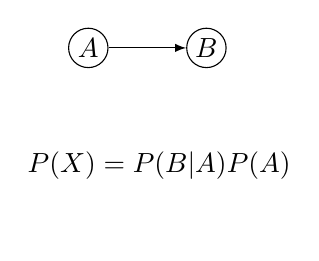
\begin{tikzpicture}[mytikzgraphoptions]

    % nodes
    \node (a) at (0,0)  {$\mysnl{A}$};
    \node (b) at (5,0)  {$\mysnl{B}$};
    \textnode at (3,-5)  {$P(X) = P(B|A)P(A)$};
    \textnode at (0,-7)  {};

    % edges
    \draw (a) edge (b);
\end{tikzpicture}



        \caption{Bayesian network.}
        \label{subfig:bn}
    \end{subfigure}\hfill
    \begin{subfigure}[b]{80pt}
        \centering
        \scalebox{0.9}{
        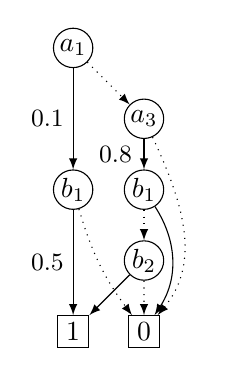
\begin{tikzpicture}[mytikzbddoptions]

    % nodes
    \node (a1) at (0,-3)     {$a_1$};
    \node (a3) at (3,-6) {$a_3$};
    \node (b1) at (0,-9)  {$b_1$};
    \node (b12) at (3,-9)  {$b_1$};
    \node (b22) at (3,-12)  {$b_2$};

    \terminalnode (false) at (3,-15) {$0$};
    \terminalnode (true) at (0,-15)   {$1$};

    % edges
    \draw[dotted] (a1) edge (a3);
    \draw[dotted,in=50,out=-65] (a3) edge (false);
    \draw[bend right=10,dotted] (b1) edge (false);
    \draw[dotted] (b12) edge (b22);
    \draw[dotted] (b22) edge (false);

    \draw  (a1)   edge node[draw=none,midway,left,xshift=-2]  {\mytikzsmallfontsize{$0.1$}}(b1);
    \draw  (a3)   edge  node[draw=none,midway,left,xshift=-3]  {\mytikzsmallfontsize{$0.8$}}(b12);
    \draw  (b1)   edge node[draw=none,midway,left,xshift=-2]  {\mytikzsmallfontsize{$0.5$}}  (true);
    \draw[bend left=33]  (b12)  edge (false);
    \draw  (b22)  edge  (true);
\end{tikzpicture}


        }

        \caption{BDD.}
        \label{subfig:bdd}
    \end{subfigure}\hfill


    \caption{Bayesian network with local structure.}
    \label{fig:bn}
\end{figure}


\end{example}

Posterior probabilities can be computed using well-known lemmas in probability theory, like Bayes’ theorem:
\[P(X | Y) = \frac{P(X | Y)P(Y)}{P(Y)},\]
marginalization $P(X) = \sum_{y} P(X, Y = y)$, and the factorization property (Defintion~\ref{def:bnfac}).



%!TEX root = main.tex

\section{Probabilistic Inference using Decision Diagrams}\label{sec:parallel}


Bayesian networks represent concise factorizations of a probability distribution by using conditional independence assumptions. The size of the factorization has direct implications toward the cost of reasoning, i.e., probabilitic inference. A more expressive model must be used to further improve a BN's factorization in order to exploit additional independences~\cite{boutilier1996context,friedman1998learning,zhang1996exploiting}. A prominent way of achieving this is by using Boolean algebra to find a more concise and canonical representation, such as a Binary Decision Diagrams (BDD). Compiling a BN into a BDD-like representations is commonly referred to as \emph{knowledge compilation}~\cite{darwiche2002knowledge}, or simply compilation.

\begin{figure}[!t]
    \centering
    \scalebox{0.9}{
        \begin{minipage}[!]{\mytikzfigurewidth}
    \centering
    \begingroup
    \usetikzlibrary{fit}
    \tikzsetnextfilename{\mytikzfigurekey}
    \begin{tikzpicture}[scale=1.6*\mytikzscale,
            every path/.style={>=latex},
            inner sep=0pt,
            line width=1pt,
            thin,
            font=\mytikznormalfontsize]

        \newcommand{\myrectanglesize}{44pt}
        \newcommand{\mynodesize}{16pt}
        \newcommand{\mytikzlocalscale}{0.5}

        \begin{scope}[shift={(0,0)}]
            \node[draw,rectangle,rounded corners,solid,thin,minimum width=\myrectanglesize,minimum height=\myrectanglesize]  (bn) at (0,0)     {};


            \begin{scope}[
                shift={(0,0.7)},
                scale=\mytikzlocalscale,
                every node/.style={solid,circle,draw,minimum size=\mynodesize*\mytikzlocalscale},
                every path/.style={>=latex,->},
                ]
                \node (a) at (0,0)     {};
                \node (b) at (-2,-2.5) {};
                \node (c) at ( 2,-2.5) {};
                \draw (a) edge (b);
                \draw (a) edge (c);
            \end{scope}
        \end{scope}

        \begin{scope}[shift={(0,-5)}]
            \node[draw,rectangle,rounded corners,solid,thin,minimum width=\myrectanglesize,minimum height=\myrectanglesize]  (partitionedbn) at (0,0)     {};

            \begin{scope}[shift={(0,0.7)},scale=\mytikzlocalscale,every node/.style={draw,minimum size=\mynodesize*\mytikzlocalscale},every path/.style={>=latex}]
                \node[circle,solid] (a) at (0,0)     {};
                \node[circle,solid] (b) at (-2,-2.5) {};
                \node[circle,solid] (c) at ( 2,-2.5) {};
                \draw[->] (a) edge (b);
                \draw[->] (a) edge (c);

                \node[inner sep=2pt,rotate fit=52,rounded corners=2pt,draw,densely dashed,fit=(a) (b)]  {};
                \node[inner sep=2pt,rotate fit=52,rounded corners=2pt,draw,densely dashed,fit=(c)]  {};
            \end{scope}
        \end{scope}

        \begin{scope}[shift={(-5,-10)}]
            \node[draw,rectangle,rounded corners,solid,thin,minimum width=\myrectanglesize,minimum height=\myrectanglesize]  (component1) at (0,0)     {};

            \begin{scope}[shift={(0,0.7)},scale=\mytikzlocalscale,every node/.style={draw,minimum size=\mynodesize*\mytikzlocalscale},every path/.style={>=latex}]
                \node[circle,solid] (a) at (0,0)     {};
                \node[circle,solid] (b) at (-2,-2.5) {};
                \node[draw=none] (c) at ( 2,-2.5) {};
                \draw[->] (a) edge (b);

            \end{scope}
        \end{scope}

        \begin{scope}[shift={(5,-10)}]
            \node[draw,rectangle,rounded corners,solid,thin,minimum width=\myrectanglesize,minimum height=\myrectanglesize]  (component2) at (0,0)     {};

            \begin{scope}[shift={(0,0.7)},scale=\mytikzlocalscale,every node/.style={draw,minimum size=\mynodesize*\mytikzlocalscale},every path/.style={>=latex}]
                \node[draw=none] (a) at (0,0)     {};
                \node[draw=none] (b) at (-2,-2.5) {};
                \node[circle,solid] (c) at ( 2,-2.5) {};

            \end{scope}
        \end{scope}
        \begin{scope}[shift={(-5,-15)},every text node part/.style={align=center}]
            \node[draw,rectangle,rounded corners,solid,thin,minimum width=\myrectanglesize,minimum height=\myrectanglesize]  (cnf1) at (0,0)     {\scriptsize{Boolean}\\[-5pt]\scriptsize{formula}\\[-2pt] $f$};

        \end{scope}

        \begin{scope}[shift={(5,-15)},every text node part/.style={align=center}]
            \node[draw,rectangle,rounded corners,solid,thin,minimum width=\myrectanglesize,minimum height=\myrectanglesize]  (cnf2) at (0,0)     {\scriptsize{Boolean}\\[-5pt]\scriptsize{formula}\\[-2pt] $g$};
        \end{scope}


        \begin{scope}[shift={(-5,-20)}]
            \node[draw,rectangle,rounded corners,solid,thin,minimum width=\myrectanglesize,minimum height=\myrectanglesize]  (bdd1) at (0,0)     {};


            \begin{scope}[shift={(-0.2,1.2)},scale=\mytikzlocalscale,every node/.style={draw,minimum size=0.7*\mynodesize*\mytikzlocalscale},every path/.style={>=latex}]
                \node[circle,solid] (a) at (0,0)     {};
                \node[circle,solid] (b) at (-1,-1.5) {};
                \node[circle,solid] (c) at ( 1,-1.5) {};
                \node[circle,solid] (d) at (0,-3)     {};
                \node[circle,solid] (e) at (2,-3) {};
                \node[rectangle,solid] (true) at (0,-5) {};
                \node[rectangle,solid] (false) at (2,-5) {};

                \draw[-] (a) edge (b);
                \draw[-,densely dotted] (a) edge (c);
                \draw[-] (c) edge (d);
                \draw[-,densely dotted] (c) edge (e);
                \draw[-,bend right=20] (b) edge (true);
                \draw[-,densely dotted,bend left=20] (b) edge (false);
                \draw[-] (d) edge (true);
                \draw[-,densely dotted] (d) edge (false);
                \draw[-] (e) edge (true);
                \draw[-,densely dotted] (e) edge (false);
            \end{scope}
        \end{scope}


        \begin{scope}[shift={(5,-20)}]
            \node[draw,rectangle,rounded corners,solid,thin,minimum width=\myrectanglesize,minimum height=\myrectanglesize]  (bdd2) at (0,0)     {};

            \begin{scope}[xscale=-1,shift={(-0.2,1.2)},scale=\mytikzlocalscale,every node/.style={draw,minimum size=0.7*\mynodesize*\mytikzlocalscale},every path/.style={>=latex}]
                \node[circle,solid] (a) at (0,0)     {};
                \node[circle,solid] (b) at (-1,-1.5) {};
                \node[circle,solid] (c) at ( 1,-1.5) {};
                \node[circle,solid] (d) at (0,-3)     {};
                \node[circle,solid] (e) at (2,-3) {};
                \node[rectangle,solid] (true) at (0,-5) {};
                \node[rectangle,solid] (false) at (2,-5) {};

                \draw[-] (a) edge (b);
                \draw[-,densely dotted] (a) edge (c);
                \draw[-] (c) edge (d);
                \draw[-,densely dotted] (c) edge (e);
                \draw[-,bend right=20] (b) edge (true);
                \draw[-,densely dotted,bend left=20] (b) edge (false);
                \draw[-] (d) edge (true);
                \draw[-,densely dotted] (d) edge (false);
                \draw[-] (e) edge (true);
                \draw[-,densely dotted] (e) edge (false);
            \end{scope}
        \end{scope}

        \begin{scope}[shift={(0,-30)}]
            \newcommand{\mycomposedscale}{3.2}
            \node[draw,rectangle,rounded corners,solid,thin,minimum width=\mycomposedscale*\myrectanglesize,minimum height=\mycomposedscale*\myrectanglesize]  (composed) at (0,0)     {};

            \begin{scope}[shift={(0,\mycomposedscale)}]
                \node[draw,rectangle,rounded corners,densely dashed,thin,minimum width=\myrectanglesize,minimum height=\myrectanglesize]  (composed1) at (0,0)     {};

                \begin{scope}[shift={(-0.2,1.2)},scale=\mytikzlocalscale,every node/.style={draw,minimum size=0.7*\mynodesize*\mytikzlocalscale},every path/.style={>=latex}]
                    \node[circle,solid] (a) at (0,0)     {};
                    \node[circle,solid] (b) at (-1,-1.5) {};
                    \node[circle,solid] (c) at ( 1,-1.5) {};
                    \node[circle,solid] (d) at (0,-3)     {};
                    \node[circle,solid] (e) at (2,-3) {};
                    \node[rectangle,solid] (true) at (0,-5) {};
                    \node[rectangle,solid] (false) at (2,-5) {};

                    \draw[-] (a) edge (b);
                    \draw[-,densely dotted] (a) edge (c);
                    \draw[-] (c) edge (d);
                    \draw[-,densely dotted] (c) edge (e);
                    \draw[-,bend right=20] (b) edge (true);
                    \draw[-,densely dotted,bend left=20] (b) edge (false);
                    \draw[-] (d) edge (true);
                    \draw[-,densely dotted] (d) edge (false);
                    \draw[-] (e) edge (true);
                    \draw[-,densely dotted] (e) edge (false);
                \end{scope}
            \end{scope}
            \begin{scope}[shift={(\mycomposedscale,-\mycomposedscale)}]
                \node[draw,rectangle,rounded corners,densely dashed,thin,minimum width=\myrectanglesize,minimum height=\myrectanglesize]  (composed2) at (0,0)     {};

                \begin{scope}[xscale=-1,shift={(-0.2,1.2)},scale=\mytikzlocalscale,every node/.style={draw,minimum size=0.7*\mynodesize*\mytikzlocalscale},every path/.style={>=latex}]
                    \node[circle,solid] (a) at (0,0)     {};
                    \node[circle,solid] (b) at (-1,-1.5) {};
                    \node[circle,solid] (c) at ( 1,-1.5) {};
                    \node[circle,solid] (d) at (0,-3)     {};
                    \node[circle,solid] (e) at (2,-3) {};
                    \node[rectangle,solid] (true) at (0,-5) {};
                    \node[rectangle,solid] (false) at (2,-5) {};

                    \draw[-] (a) edge (b);
                    \draw[-,densely dotted] (a) edge (c);
                    \draw[-] (c) edge (d);
                    \draw[-,densely dotted] (c) edge (e);
                    \draw[-,bend right=20] (b) edge (true);
                    \draw[-,densely dotted,bend left=20] (b) edge (false);
                    \draw[-] (d) edge (true);
                    \draw[-,densely dotted] (d) edge (false);
                    \draw[-] (e) edge (true);
                    \draw[-,densely dotted] (e) edge (false);
                \end{scope}
            \end{scope}
            \begin{scope}[shift={(-\mycomposedscale,-\mycomposedscale)}]
                \node[draw,rectangle,rounded corners,densely dashed,thin,minimum width=\myrectanglesize,minimum height=\myrectanglesize]  (composed3) at (0,0)     {};

                \begin{scope}[xscale=-1,shift={(-0.2,1.2)},scale=\mytikzlocalscale,every node/.style={draw,minimum size=0.7*\mynodesize*\mytikzlocalscale},every path/.style={>=latex}]
                    \node[circle,solid] (a) at (0,0)     {};
                    \node[circle,solid] (b) at (-1,-1.5) {};
                    \node[circle,solid] (c) at ( 1,-1.5) {};
                    \node[circle,solid] (d) at (0,-3)     {};
                    \node[circle,solid] (e) at (2,-3) {};
                    \node[rectangle,solid] (true) at (0,-5) {};
                    \node[rectangle,solid] (false) at (2,-5) {};

                    \draw[-] (a) edge (b);
                    \draw[-,densely dotted] (a) edge (c);
                    \draw[-] (c) edge (d);
                    \draw[-,densely dotted] (c) edge (e);
                    \draw[-,bend right=20] (b) edge (true);
                    \draw[-,densely dotted,bend left=20] (b) edge (false);
                    \draw[-] (d) edge (true);
                    \draw[-,densely dotted] (d) edge (false);
                    \draw[-] (e) edge (true);
                    \draw[-,densely dotted] (e) edge (false);
                \end{scope}
            \end{scope}

            \draw[->,densely dashed] (composed1) edge (composed2);
            \draw[->,densely dashed] (composed1) edge (composed3);
        \end{scope}

        % edges
        \draw[->] (bn) edge (partitionedbn);
        \draw[->,shorten >= -2pt, shorten <= -2pt] (partitionedbn) edge (component1);
        \draw[->,shorten >= -2pt, shorten <= -2pt] (partitionedbn) edge (component2);
        \draw[->] (component1) edge (cnf1);
        \draw[->] (component2) edge (cnf2);
        \draw[->] (cnf1) edge (bdd1);
        \draw[->] (cnf2) edge (bdd2);
        \draw[->] (bdd1) edge (composed);
        \draw[->] (bdd2) edge (composed);

        %% independence edge
        %\begin{scope}[every path/.style={
        %        >=stealth,
        %        decoration = {snake,pre length=7pt,post length=9pt},
        %        decorate,
        %        densely dashed,
        %        shorten >= 4pt, shorten <= 4pt}]

        %        \usetikzlibrary{arrows, decorations.pathmorphing}

        %        \draw[<->] (component1) -- (component2);
        %        \draw[<->] (cnf1) -- (cnf2);
        %        \draw[<->] (bdd1) -- (bdd2);
        %        \draw[<->,shorten >= 0.5pt, shorten <= 0.5pt,decoration = {snake,pre length=3pt,post length=2pt}] (composed2) -- (composed3);
        %        \begin{scope}[shift={(1.5,-0.5)}]
        %            \draw[<->,decoration = {snake,pre length=7pt,post length=6pt},] (7,-33.5) -- node[rectangle,inner sep=0pt,draw=none,midway,yshift=-\myfontsize] {Independencies} (14,-33.5);
        %        \end{scope}

        %\end{scope}
        %\node[draw,rectangle,rounded corners,densely dotted,thin,minimum width=60pt,minimum height=30pt] (x) at (12,-34.7)     {};

        \begin{scope}[every node/.style={
                rotate=45,
                draw=none,
                anchor=west,
                align=left}]
            %\draw[-,dotted,shorten >= 10pt, shorten <= 10pt] (bn) -- (8,0);
            %\draw[-,dotted,shorten >= 10pt, shorten <= 10pt] (partitionedbn) -- (8,-5);
            \usetikzlibrary{calc}
            \textnode (bnlabel) at (10,0) {Bayesian\\Network};
            \draw[-,densely dotted,shorten >= 5pt, shorten <= 5pt] (bn) -- (bnlabel.west);

            \textnode (partitionlabel) at (10,-5) {Partitioning};
            \draw[-,densely dotted,shorten >= 5pt, shorten <= 5pt] (partitionedbn) -- (partitionlabel.west);
            \draw[-,rounded corners,densely dotted,shorten <= 5pt] (component2) -- ($(component2)+(3.4,0)$) --  ($(partitionedbn)+(8.4,0)$);

            \textnode  (encodinglabel) at (10,-15) {Encoding};
            \draw[-,densely dotted,shorten >= 5pt, shorten <= 5pt] (cnf2) -- (encodinglabel.west);

            \textnode  (compilationlabel) at (10,-20) {Decision\\ Diagrams};
            \draw[-,densely dotted,shorten >= 5pt, shorten <= 5pt] (bdd2) -- (compilationlabel.west);

            \textnode  (compositionlabel) at (10,-30) {Composed\\Representation};
            \draw[-,densely dotted,shorten >= 5pt, shorten <= 5pt] (composed) -- (compositionlabel.west);
        \end{scope}

        \draw[-,densely dotted] (-7,2.5) -- (-8,2.5) -- (-8,-22.5) node[rectangle,inner sep=0pt,draw=none,rotate=90,midway,yshift=8pt] {Compilation} -- (-7,-22.5);
        \draw[-,densely dotted] (-7,-23.5) -- (-8,-23.5)  -- (-8,-36.5) node[rectangle,inner sep=0pt,draw=none,rotate=90,midway,yshift=8pt] {Inference} -- (-7,-36.5);
\end{tikzpicture}
\endgroup
\end{minipage}

    }
    \caption{The compositional framework.}
    \label{fig:frameworkoverview}
\end{figure}


Figure~\ref{fig:frameworkoverview} shows an overview of the underlying principles behind probablistic inference using BDDs, divided into two steps: \emph{compilation} and \emph{inference}. We will dive into these steps in the following sections without going into too much detail. In-depth descriptions can be found in~\cite{dal2021compositional}.

\subsection{Compilation}

We first describe compilation as being all steps required to obtain a BDD. In addition to traditional compilation, we introduce partitioning to further improve overall performance~\cite{dal2017reducing}.

A partitioning is found for the BN. This partitioning is optimized by minimizing the sum of each partition's tree-width. Tree-width is a metric commonly used to indicate the complexity of BNs~\cite{bollig2014width}. With the partitioning in hand, the following steps can be performed independently, per partition. Theoretically, compilation is as fast as the slowest compiling partition~\cite{dal2018parallel}. Each partition is considered an independent BN from this point on.

BNs are defined over multi-valued domains. Prior to compiling it to a BDD, we require an encoding to transition from the multi-valued domain to the Boolean domain. There are multiple ways to do this. We chooses to first translate a BN into a satisfiability (SAT) instance in Conjunctive Normal Form (CNF) with dedicated variables to represent probabilities~\cite{chavira2008probabilistic,dal2017wpbdd} (in this step we do not need to introduce extra variables as e.g. a Tseitin transformation would).

The obtained SAT instance serves as an entry point into the field of language compilers~\cite{dudek2020addmc}. These compilers target different variations of BDDs. The process of compiling a SAT instance to a respective BDD using one such compiler is by far the most expensive operation of the entire process. Performance is primarily determined by this step, while inference if mich cheaper.

With monolithic compilation, we would only be able to amortize cost of compilation by performing many inference queries. With partitioned compilation, we shift some of this cost over to the inference side, yielding overall performance improvements in cases where we would traditionally not be able to achieve sufficient amortization~\cite{dal2017reducing}. We have now reached the end of the compilation part as indicated by Figure~\ref{fig:frameworkoverview}.

\subsection{Inference}

After compilation we arrive at the inference step. The upside of getting this far, is that the computational complexity of inference is linear in the size of the target representation~\cite{darwiche2002knowledge}. Inference is performed by traversing the target representation whilst evaluating the underlying arithmetic formula. The arithmetic formula is different for every target representation, but generally we can convert a logical OR to addition, logical AND to multiplication, and substitute variables with the value or probability they represent. All that is left, is to evaluate this formula in order to obtain the marginal probability we seek. In short, this is inference by \emph{Weighted Model Counting} (WMC)~\cite{chavira2008probabilistic}.

In case we chose to partition the BN during the compilation step, we have to compose the compiled BDDs and create a monolithic representation. A partition's representation is connected to another of they share a common variable. This implies that the order in which we traverse partitions is not a total ordering, it is partial. It can be represented by a tree, we suitably refer to as a composition-tree~\cite{dal2021compositional}. The order in which we choose to traverse partitions determines how they are connected. As we traverse one partition, its sink is connected to the next partition's root. Now that all partitions form one connected component, we can proceed as previous described with a traversal we are already familier with from WMC.


\section{\toolname}

\begin{figure}[!t]
    \centering
    \begin{minipage}[!]{\mytikzfigurewidth}
    \centering
    \begingroup
    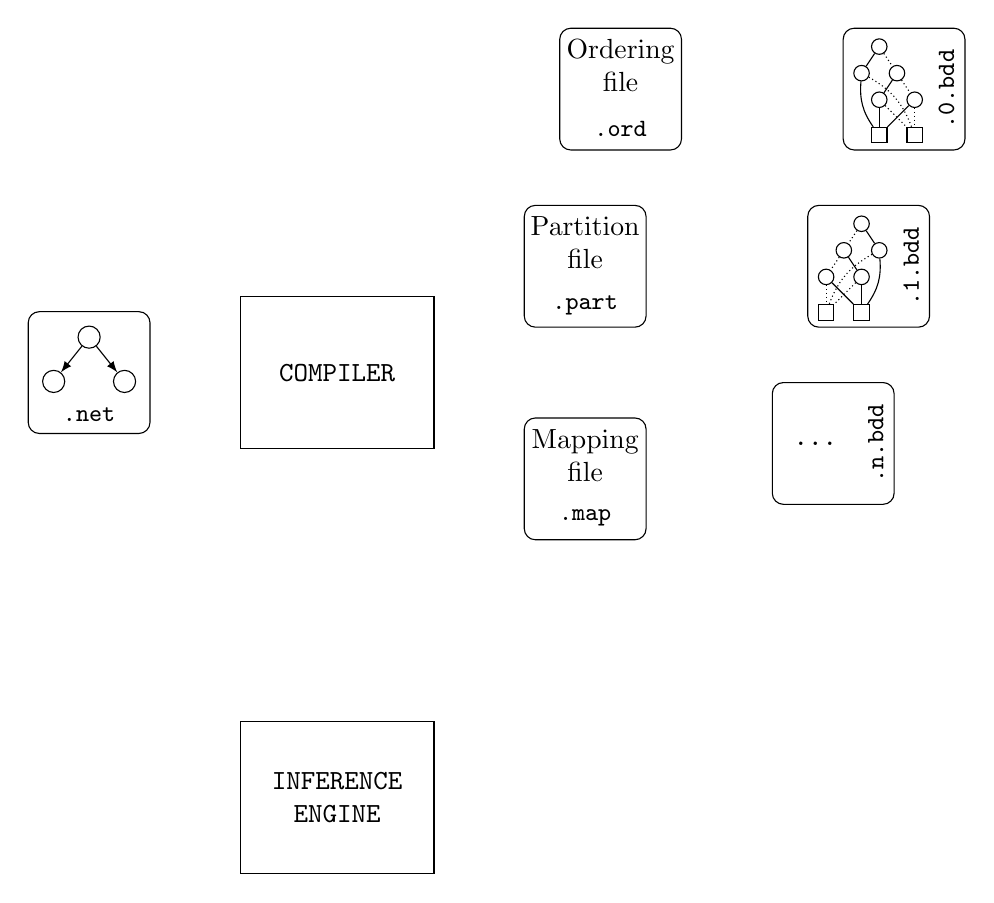
\begin{tikzpicture}[scale=1.5*\mytikzscale,
            every path/.style={>=latex},
            inner sep=0pt,
            line width=1pt,
            thin,
            font=\mytikznormalfontsize]

        \newcommand{\myrectanglesize}{44pt}
        \newcommand{\mynodesize}{16pt}
        \newcommand{\mytikzlocalscale}{0.5}

        % bayesian network input
        \begin{scope}[shift={(0,0)}]
            \node[draw,rectangle,rounded corners,solid,thin,minimum width=\myrectanglesize,minimum height=\myrectanglesize]  (bn) at (0,0)     {};


            \begin{scope}[
                shift={(0,1)},
                scale=\mytikzlocalscale,
                every node/.style={solid,circle,draw,minimum size=\mynodesize*\mytikzlocalscale},
                every path/.style={>=latex,->},
                ]
                \node (a) at (0,0)     {};
                \node (b) at (-2,-2.5) {};
                \node (c) at ( 2,-2.5) {};
                \draw (a) edge (b);
                \draw (a) edge (c);
            \end{scope}
            \textnode (bnlabel) at (0,-1.2) {\small\verb+.net+};
        \end{scope}


        % compiler
        \begin{scope}[shift={(7,0)},every text node part/.style={align=center}]
            \node[draw,rectangle,solid,thin,minimum width=70pt,minimum height=55pt]  (compiler) at (0,0)     {\verb+COMPILER+};

        \end{scope}

        % inference engine
        \begin{scope}[shift={(7,-12)},every text node part/.style={align=center}]
            \node[draw,rectangle,solid,thin,minimum width=70pt,minimum height=55pt]  (inference) at (0,0)     {\verb+INFERENCE+\\\verb+ENGINE+};

        \end{scope}

        % ordering file
        \begin{scope}[shift={(15,8)}]
            \node[draw,rectangle,rounded corners,solid,thin,minimum width=\myrectanglesize,minimum height=\myrectanglesize]  (ordering) at (0,0)     {};

            \textnode[align=center, shift={(0,0.3)}] {Ordering\\file};
            \textnode[shift={(0,-0.5)}] {\small \verb+.ord+};
        \end{scope}

% partition file
        \begin{scope}[shift={(14,3)}]
            \node[draw,rectangle,rounded corners,solid,thin,minimum width=\myrectanglesize,minimum height=\myrectanglesize]  (partition) at (0,0)     {};
            \textnode[align=center, shift={(0,0.3)}] {Partition\\file};
            \textnode[shift={(0,-0.5)}] {\small \verb+.part+};
        \end{scope}

        % mapping file
        \begin{scope}[shift={(14,-3)}]
            \node[draw,rectangle,rounded corners,solid,thin,minimum width=\myrectanglesize,minimum height=\myrectanglesize]  (mapping) at (0,0)     {};

            \textnode[align=center, shift={(0,0.3)}] {Mapping\\file};
            \textnode[shift={(0,-0.5)}] {\small \verb+.map+};
        \end{scope}


        % first BDD
        \begin{scope}[shift={(23,8)}]
            \node[draw,rectangle,rounded corners,solid,thin,minimum width=\myrectanglesize,minimum height=\myrectanglesize]  (bdd1) at (0,0)     {};

            \textnode[rotate=90] (bdd1label) at (1.2,0) {\small\verb+.0.bdd+};

            \begin{scope}[shift={(-0.7,1.2)},scale=\mytikzlocalscale,every node/.style={draw,minimum size=0.7*\mynodesize*\mytikzlocalscale},every path/.style={>=latex}]
                \node[circle,solid] (a) at (0,0)     {};
                \node[circle,solid] (b) at (-1,-1.5) {};
                \node[circle,solid] (c) at ( 1,-1.5) {};
                \node[circle,solid] (d) at (0,-3)     {};
                \node[circle,solid] (e) at (2,-3) {};
                \node[rectangle,solid] (true) at (0,-5) {};
                \node[rectangle,solid] (false) at (2,-5) {};

                \draw[-] (a) edge (b);
                \draw[-,densely dotted] (a) edge (c);
                \draw[-] (c) edge (d);
                \draw[-,densely dotted] (c) edge (e);
                \draw[-,bend right=20] (b) edge (true);
                \draw[-,densely dotted,bend left=20] (b) edge (false);
                \draw[-] (d) edge (true);
                \draw[-,densely dotted] (d) edge (false);
                \draw[-] (e) edge (true);
                \draw[-,densely dotted] (e) edge (false);
            \end{scope}
        \end{scope}

        % second BDD
        \begin{scope}[shift={(22,3)}]
            \node[draw,rectangle,rounded corners,solid,thin,minimum width=\myrectanglesize,minimum height=\myrectanglesize]  (bdd2) at (0,0)     {};

            \textnode[rotate=90] (bdd2label) at (1.2,0) {\small\verb+.1.bdd+};

            \begin{scope}[xscale=-1,shift={(0.2,1.2)},scale=\mytikzlocalscale,every node/.style={draw,minimum size=0.7*\mynodesize*\mytikzlocalscale},every path/.style={>=latex}]
                \node[circle,solid] (a) at (0,0)     {};
                \node[circle,solid] (b) at (-1,-1.5) {};
                \node[circle,solid] (c) at ( 1,-1.5) {};
                \node[circle,solid] (d) at (0,-3)     {};
                \node[circle,solid] (e) at (2,-3) {};
                \node[rectangle,solid] (true) at (0,-5) {};
                \node[rectangle,solid] (false) at (2,-5) {};

                \draw[-] (a) edge (b);
                \draw[-,densely dotted] (a) edge (c);
                \draw[-] (c) edge (d);
                \draw[-,densely dotted] (c) edge (e);
                \draw[-,bend right=20] (b) edge (true);
                \draw[-,densely dotted,bend left=20] (b) edge (false);
                \draw[-] (d) edge (true);
                \draw[-,densely dotted] (d) edge (false);
                \draw[-] (e) edge (true);
                \draw[-,densely dotted] (e) edge (false);
            \end{scope}
        \end{scope}

        % third BDD
        \begin{scope}[shift={(21,-2)}]
            \node[draw,rectangle,rounded corners,solid,thin,minimum width=\myrectanglesize,minimum height=\myrectanglesize]  (bdd2) at (0,0)     {};

            \textnode[rotate=90] (bddnlabel) at (1.2,0) {\small\verb+.n.bdd+};
            \textnode[] (bddntag) at (-0.5,0) {\verb+...+};


        \end{scope}


        \begin{scope}[every node/.style={
                rotate=45,
                draw=none,
                anchor=west,
                align=left}]
            %\draw[-,dotted,shorten >= 10pt, shorten <= 10pt] (bn) -- (8,0);
            %\draw[-,dotted,shorten >= 10pt, shorten <= 10pt] (partitionedbn) -- (8,-5);
            \usetikzlibrary{calc}


        \end{scope}

\end{tikzpicture}
\endgroup
\end{minipage}

    \caption{The implementation.}
    \label{fig:implementation}
\end{figure}


%Figure~\ref{fig:frameworkoverview} shows a high level overview of the tool's internal processes.
%
%A partitioning is found for the BN. This partitioning is optimized by minimizing the sum of each partition's tree-width. Tree-width is a metric commonly use to indicate the complexity of BNs~\cite{bollig2014width}.
%
% using \emph{simulated annealing}
%
%
% The \toolname compiler however specifically targets \emph{Weighted Positive Binary Decision Diagrams} (WPBDD), which is a dedicated representation for probabilistic inference. (We discuss differences with other representations in Section~\ref{sec:conclusion}.) In addition, the compiler introduces a partitioning to further improve overall performance~\cite{dal2017reducing}.
%
%
%\toolname takes this Boolean formula and compiles it to a WPBDD.          , yielding a WPBDD per partition
%
%
%is that the computational complexity of inference is linear in the size of the target representation~\cite{darwiche2002knowledge}, in our case a WPBDD.
%
%
%
%With the partitioning in hand, the following steps can be performed in parallel, per partition. Theoretically, compilation is as fast as the slowest compiling partition~\cite{dal2018parallel}.
%



%!TEX root = main.tex

\section{Tool Usage}
\label{sec:usage}


\todo[inline]{
Give command lines and explain rational

Perhaps with an example? A simple network?
}


%%!TEX root = main.tex

\section{Experiments}
\label{sec:experiments}


%%!TEX root = main.tex

\section{Related Work}
\label{sec:related}

%!TEX root = main.tex

\section{Discussion}
\label{sec:conclusion}

\toolname shows that parallelism can benefit knowledge compilation and inference for Bayesian networks. Our chosen parallelization approach is based on partitioning. An approach that has previously been exploited to speed up symbolic model checking~\cite{grumberg2006work,narayan1996partitioned,sahoo2004partitioning}.  We additionally find that the partitioning introduces a tradeoff between compilation times and inference times, sacrificing some performance in inference to gain parallel scalability.

The computational complexity of inference is linear in the size of the target representation~\cite{darwiche2002knowledge}. However, it increases when partitioning is employed. A compiled partition in a composition-tree must be exponentially traversed in the size of the cutset that separates it from its parent. Once for every instantiation of the curset variables. However, this is compensated by a number of principles. $(1)$ the combined size of all partition BDDs is significantly reduced compared to the monolithicly compiled BDD~\cite{dal2017reducing}; $(2)$ partition BDDs only represent a portion of its total, reducing traversal resources; $(3)$ each child instantiation can be traversed in parallel, potentially reducing traversal cost of exponential traversals to the cost of 1~\cite{dal2021compositional}; $(4)$ as partition BDDs are small, cache locality start to play an important role, giving an advantage over monolithic BDDs~\cite{dal2018parallel}. Beyond the complexity introduced by cutsets, inference remains linear. Small cutsets can therefore play a crucial role in performance. Seperate empirical investigations on partitioning and parallelism show their respective contributation to \toolname's performance~\cite{dal2018parallel,dal2021compositional}.


\todo[inline]{
Discuss other tools in more details (ACE, dlib, etc)
}

The parallization approach of \toolname is orthogonal to the chosen target representation of the knowledge base, which we demonstrated by using it for four different target representations~\cite{dal2018parallel}. As a consequence, the approach is to a certain extent orthogonal to the exploitation of local structure~\cite{chavira2005compiling} by those representations, as local structure can still be exploited within the partitioned subproblems. For instance, we showed that causal dependence is fully exploited when using decision diagram representations in the partitions.\todo{references}

For target representations, many choices exist~\cite{darwiche2001decomposable,darwiche2011sdd,darwiche2002knowledge,fargier2014knowledge}. Since our partitioning technique exploits the treewidth~\cite{dechter1998bucket} of the representation~\cite[\S 5]{dal2021compositional}, and the algorithms are based on message passing~\cite[\S 4]{dal2021compositional}, other representations like ADD and d-DNNF can be parallelized alike. While our earlier work~\cite{dal2018parallel} compared the performance of \toolname against various of these other representations, showing competitive performance, here we will point out some differences between the other representations and suggest future work.


Like AADD~\cite{sanner2005affine}, and its similar cousins SLDD~\cite{wilson2005decision}, QMDD~\cite{miller2006qmdd} and FEVBDD~\cite{tafertshofer1997factored}, our target representation WPBDD factors out probabilities on the edges of the diagram, resulting in more succinctness than for instance achieved with ADD~\cite{bahar}, QuiDD~\cite{viamontes2003improving} and MTDD~\cite{Clarke2001}. However, unlike AADD, it only factors according to the structure of the Bayesian network, which sacrifices succinctness but ensures exact representation of the floating point numbers. The latter can be quite important in practice, as rounding errors from manipulation operations can quickly propagate in the discrete data structure, resulting in numerical instability~\cite{zulehner2019efficiently}.

The effects of different variable orders is known to be crucial in many representation languages. Representations like FBDD~\cite{wegener2000branching}, d-DNNF~\cite{chavira2006compiling} and SDD~\cite{darwiche2011sdd}, allow more freedom in the order and could potentially improve the results of \toolname.\todo{we compare already favoray with sdd?}

Early versions of \toolname also tried different parallelization approaches, like the fine-grained task-based scheduling of Sylvan~\cite{van2013multi}, which has shown that good parallel scalability is possible for model checking problems in BDDs, ADDs (also called Multi-Terminal DDs), and MDDs (Sylvan uses a version called List DD~\cite{sylvan-journal}). In future work, we hope to establish why this approach did not yield good performance for knowledge compilation as well.





\todo{make citations more up to date. more citations from 2022 and 2021}

\bibliographystyle{plain}
\bibliography{lit}

%\clearpage
%%!TEX root = main.tex
 
\appendix

\section{Dynamic Reduction}
\label{app:proofs}



\end{document}

%%% Local Variables:
%%% mode: latex
%%% TeX-master: t
%%% End:
